\documentclass[compress]{beamer}
\usepackage{ifthen,verbatim}

\newcommand{\isnote}{}
\xdefinecolor{lightyellow}{rgb}{1.,1.,0.25}
\xdefinecolor{darkblue}{rgb}{0.1,0.1,0.7}

%% Uncomment this to get annotations
%% \def\notes{\addtocounter{page}{-1}
%%            \renewcommand{\isnote}{*}
%% 	   \beamertemplateshadingbackground{lightyellow}{white}
%%            \begin{frame}
%%            \frametitle{Notes for the previous page (page \insertpagenumber)}
%%            \itemize}
%% \def\endnotes{\enditemize
%% 	      \end{frame}
%%               \beamertemplateshadingbackground{white}{white}
%%               \renewcommand{\isnote}{}}

%% Uncomment this to not get annotations
\def\notes{\comment}
\def\endnotes{\endcomment}

\setbeamertemplate{navigation symbols}{}
\setbeamertemplate{headline}{\mbox{ } \hfill
\begin{minipage}{5.5 cm}
\vspace{-0.75 cm} \small
\end{minipage} \hfill
\begin{minipage}{4.5 cm}
\vspace{-0.75 cm} \small
\begin{flushright}
\ifthenelse{\equal{\insertpagenumber}{1}}{}{Jim Pivarski \hspace{0.2 cm} \insertpagenumber\isnote/\pageref{numpages}}
\end{flushright}
\end{minipage}\mbox{\hspace{0.2 cm}}\includegraphics[height=1 cm]{../cmslogo} \hspace{0.1 cm} \includegraphics[height=1 cm]{../tamulogo} \hspace{0.01 cm} \vspace{-1.05 cm}}

\begin{document}
\begin{frame}
\vfill
\begin{center}
\textcolor{darkblue}{\Large Alignment of Endcap Stations in CRUZET}

\vfill
\begin{columns}
\column{0.3\linewidth}
\begin{center}
\large
\textcolor{darkblue}{Jim Pivarski}

\vspace{0.2 cm}
Alexei Safonov
\end{center}

\column{0.3\linewidth}
\begin{center}
\large
K\'aroly Banicz
\end{center}
\end{columns}

\begin{columns}
\column{0.3\linewidth}
\begin{center}
\scriptsize
{\it Texas A\&M University}
\end{center}
\column{0.3\linewidth}
\begin{center}
\scriptsize
{\it US-CMS}
\end{center}
\end{columns}

\vfill
31 July, 2008

\end{center}
\end{frame}

%% \begin{notes}
%% \item This is the annotated version of my talk.
%% \item If you want the version that I am presenting, download the one
%% labeled ``slides'' on Indico (or just ignore these yellow pages).
%% \item The annotated version is provided for extra detail and a written
%% record of comments that I intend to make orally.
%% \item Yellow notes refer to the content on the {\it previous} page.
%% \item All other slides are identical for the two versions.
%% \end{notes}

\begin{frame}
\frametitle{News}

Completed alignment of endcap stations in CRUZET-2;

CRUZETs 1 and 3 are in the pipeline

\vfill
\hspace{-0.83 cm} \textcolor{darkblue}{\Large Outline}

\vspace{0.2 cm}
\begin{itemize}\setlength{\itemsep}{0.5 cm}
\item How the alignment was done
\item How to access the new constants
\item Next steps
\end{itemize}
\end{frame}

\begin{frame}
\frametitle{Station-by-station alignment}

Treat each station (including rings) as a rigid body, find optimal
position using tracks from barrel and other stations
\begin{itemize}
\item Largest and most important part of alignment, improves track residuals by many centimeters
\end{itemize}

\vfill
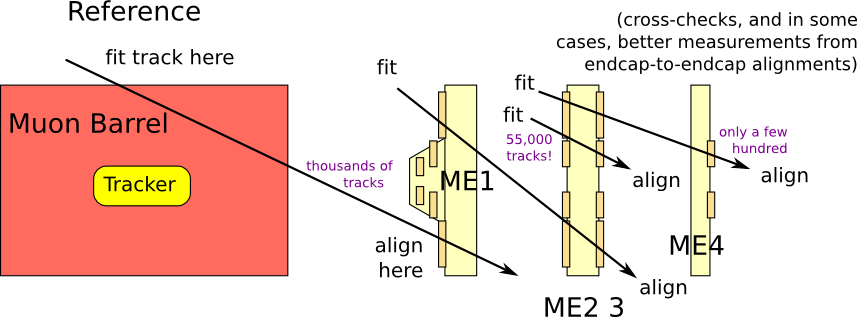
\includegraphics[width=\linewidth]{fit_here_align_there.png}

\vfill Similar to the ``baseline'' procedure for collisions data,
except that the muon barrel is the reference, rather than the tracker
\end{frame}

\begin{frame}
\frametitle{Use of HIP derivatives}
\small

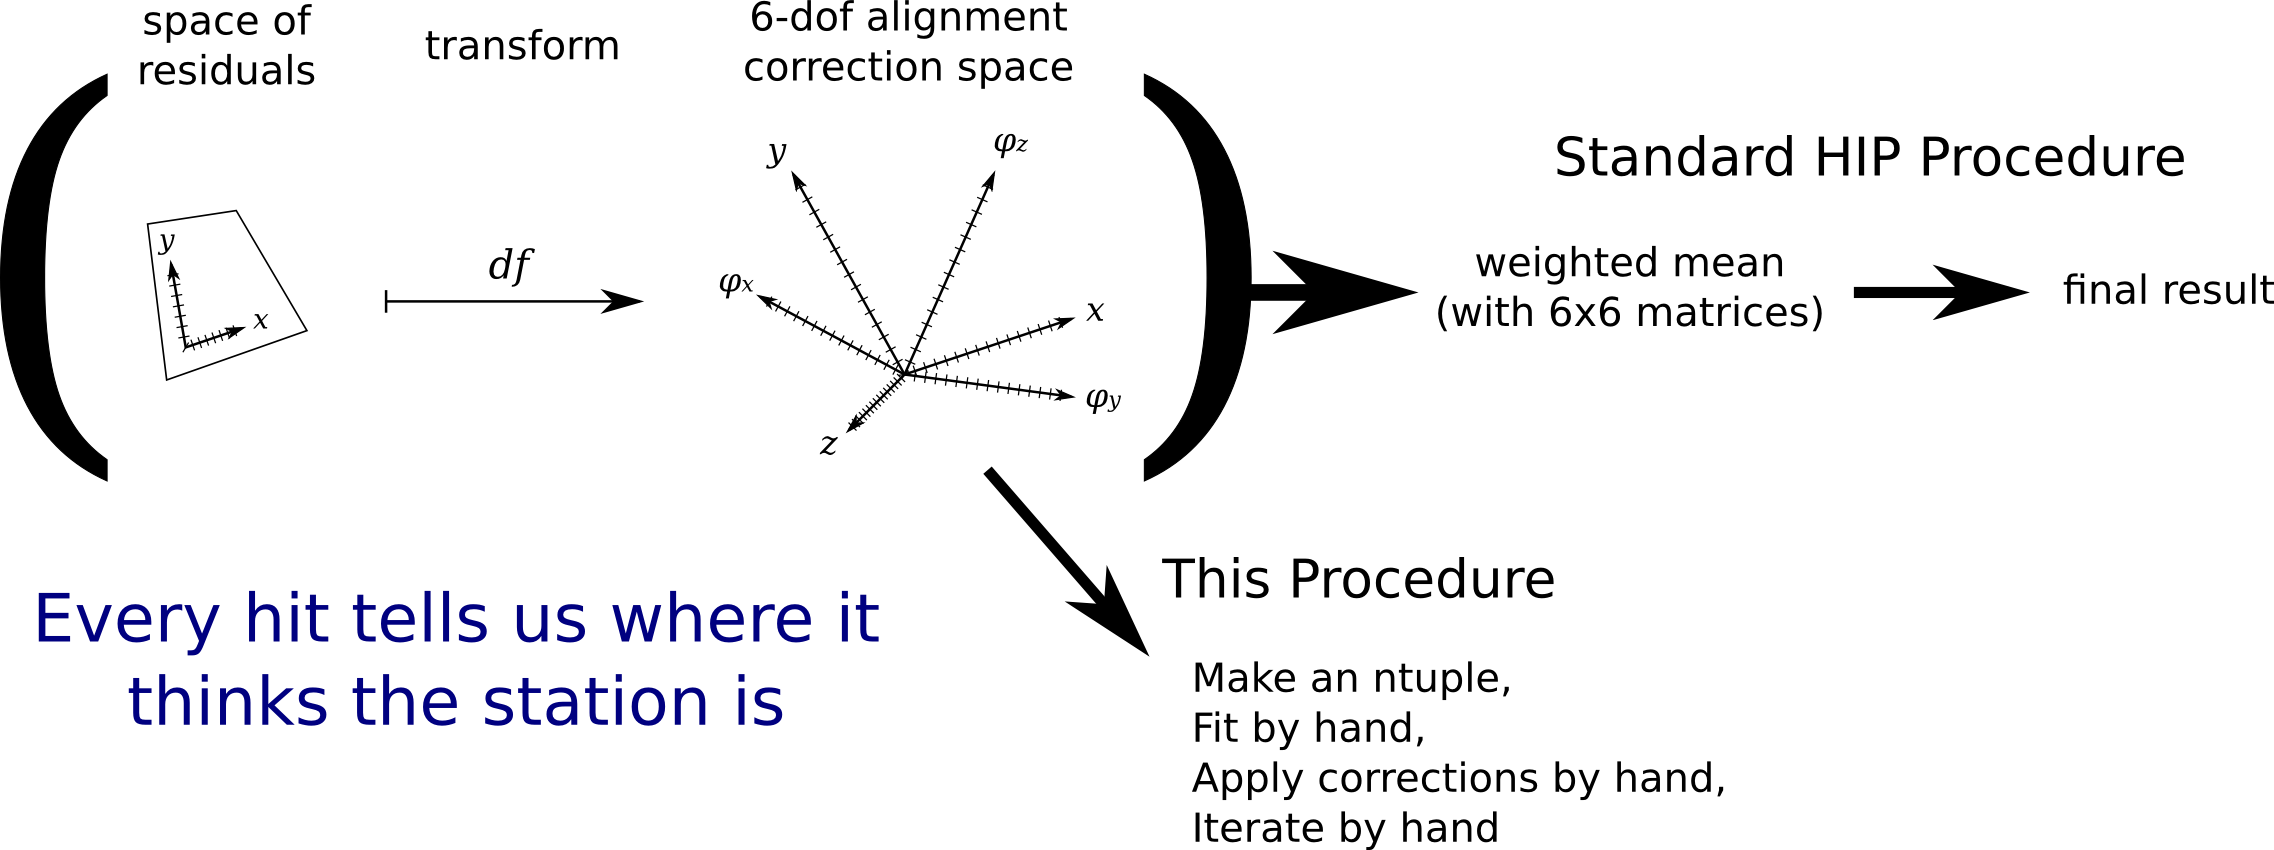
\includegraphics[width=\linewidth]{transformation.png}

\begin{columns}
\column{0.4\linewidth}
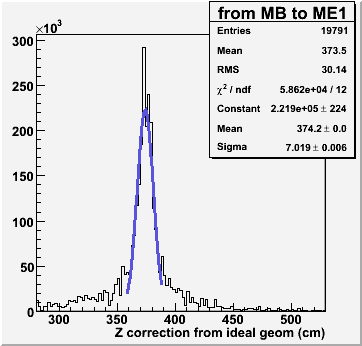
\includegraphics[width=\linewidth]{hist_0and1.png}

\column{0.65\linewidth}
Histogram of $z$ correction from every hit

\begin{itemize}
\item Without a magnetic field, can't cut on $p_T$
\item Bad tracks/hits form a broad distribution
\item Good tracks/hits agree on a $z$ position
\item Tape-measure agrees, too: 370~cm
\end{itemize}
\end{columns}
\end{frame}

\begin{frame}
\frametitle{Results at a glance:}
\hspace{-0.83 cm} \textcolor{darkblue}{\Large Where were our stations in CRUZET-2?}

\small

\vspace{0.6 cm}
\mbox{ } \hfill 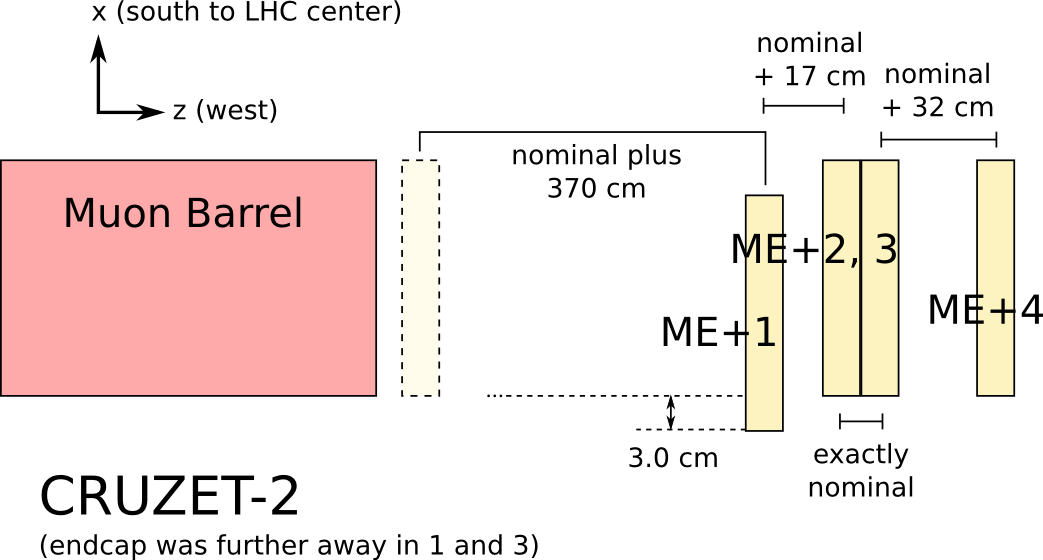
\includegraphics[width=0.9\linewidth]{where_things_are.png}

\vfill
\begin{itemize}\setlength{\itemsep}{0.1 cm}
\item Other parameters are all consistent with zero
\item Verified 370~cm opening and possibility of $\mathcal{O}($cm$)$ transverse offset
\item ``Discovered'' that ME+2 and ME+3 are mounted to the same yoke
\end{itemize}
\end{frame}

\begin{frame}
\frametitle{Internal consistency check}
\small

``MB$\to$1$\to$2'' means
\begin{itemize}
\item fit tracks in MB, use them to align ME1
\item then fit a separate set of tracks in ME1, use them to align ME2
\item should yield the same result as direct ``MB$\to$2''
\end{itemize}

\vfill
\begin{tabular}{c | c c c c}
\scriptsize Comparison & \scriptsize $x$ (mm) & \scriptsize $y$ (mm) & \scriptsize $z$ (mm) & \scriptsize $\phi_z$ (mrad) \\\hline
\scriptsize (MB$\to$2) $-$ (MB$\to$1$\to$2) & \scriptsize -12.8 $\pm$ 0.3 & \scriptsize 6.4 $\pm$ 0.4 & \scriptsize 39.9 $\pm$ 0.8 & \scriptsize -4.75 $\pm$ 0.12 \\
\scriptsize (MB$\to$3) $-$ (MB$\to$2$\to$3) & \scriptsize -3.4 $\pm$ 0.4 & \scriptsize -8.7 $\pm$ 0.5 & \scriptsize -15.3 $\pm$ 1.0 & \scriptsize -1.06 $\pm$ 0.14 \\
\scriptsize (MB$\to$4) $-$ (MB$\to$3$\to$4) & \scriptsize 0.4 $\pm$ 0.8 & \scriptsize 6.0 $\pm$ 0.9 & \scriptsize 10.3 $\pm$ 2.4 & \scriptsize 2.8 $\pm$ 0.3 \\\hline
\end{tabular}

\vfill
Statistics-only underestimates the error, but

\[ \sqrt{\frac{1}{N-1} \sum (x_i - \bar{x})^2} = \left\{\begin{array}{l} \mbox{7.8~mm for $x$ and $y$} \\ \mbox{28~mm for $z$} \\ \mbox{3.8~mrad for $\phi_z$} \end{array}\right. \]

gives a rough (over-)estimate (double-counts MB$\to$2 and MB$\to$3)
\end{frame}

\begin{frame}
\frametitle{Final values (relative to nominal)}

\small
\renewcommand{\arraystretch}{1.2}
\begin{tabular}{c | c c c c}
& $x$ (mm) & $y$ (mm) & $z$ (mm) & $\phi_z$ (mrad) \\\hline
ME+1 & -30.1038 & -3.42741 & 3736.18 & 3.2184 \\
ME+2 & 9.18771 & -18.4147 & 3910.91 & -0.466131 \\
ME+3 & 10.4957 & -15.9612 & 3911.03 & -8.88953 \\
ME+4 & 8.33082 & 0.576984 & 4227.06 & -5.60561 \\
\end{tabular} \hfill \begin{minipage}{2 cm} ($\phi_x$ and $\phi_y$ \\ set to zero) \end{minipage}

\vfill
\begin{itemize}
\item Also includes 2.5~mm outward radial correction in ME2/2 and ME3/2 to
fix error in DDD description
\end{itemize}

\vspace{-0.5 cm}
\begin{center}
\begin{minipage}{0.75\linewidth}
\tiny
\tt
\mbox{ }es\_source = PoolDBESSource \{ \\
\mbox{ }\hspace{0.5 cm}string connect = "frontier://FrontierProd/CMS\_COND\_20X\_ALIGNMENT" \\
\mbox{ }\hspace{0.5 cm}using CondDBSetup \\
\mbox{ }\hspace{0.5 cm}VPSet toGet = \{ \\
\mbox{ }\hspace{1.0 cm}\{ \\
\mbox{ }\hspace{1.5 cm}string record = "CSCAlignmentRcd" \\
\mbox{ }\hspace{1.5 cm}string tag = {\it "CRUZET2-CSCStation-xyzphiz-2mmRadialFix" } \\
\mbox{ }\hspace{1.0 cm}\} \\
\mbox{ }\hspace{0.5 cm}\} \\
\mbox{ }\} \\
\end{minipage}
\end{center}

\vspace{-0.5 cm}
\begin{itemize}
\item Track reconstruction must be performed in the same job for the alignment to take effect
\item Do not use for CRUZET-1 and 3!  (would be a 6~m error!)
\end{itemize}

\end{frame}

%% \section*{First section}
%% \begin{frame}
%% \begin{center}
%% \Huge \textcolor{blue}{First section}
%% \end{center}
%% \end{frame}

\begin{frame}
\frametitle{Next steps (short-term)}

\begin{itemize}\setlength{\itemsep}{0.3 cm}
\item Work on CRUZET-1 alignment has started
\item For CRUZET-3, we need a better sample of tracks ({\scriptsize \tt
    /Cosmics/CRUZET3\_CRUZET3\_V2P\_v3/RECO} was reconstructed with the
  6~m error; many tracks must have failed pattern-recognition)
\item A corrected CRUZET-3 re-reco begins this week, alignment will follow (finish sometime late next week?)
\item Official re-reco with fully aligned constants will come later
\item Very interesting to know how much CRUZET-2 alignment improves
  track-finding efficiency: 17 and 32~cm corrections between ME+1\&2 and ME+3\&4 are new (validation suite?)
\item Work continues on CSC-Overlaps procedure, for chamber-by-chamber
  alignments relative to the stations
\end{itemize}

\label{numpages}
\end{frame}

\end{document}
